\documentclass{class/thesis}
\usepackage{mathtools} % [draft]

%%%%%%%%%%%%%%%%%%%%%%%%%%%%%%%%%%%%%%%%%%%%%%%%
% Titel der Arbeit                             %
%%%%%%%%%%%%%%%%%%%%%%%%%%%%%%%%%%%%%%%%%%%%%%%%
\thesistitle{Facial Animation using Inverse Kinematics}

%%%%%%%%%%%%%%%%%%%%%%%%%%%%%%%%%%%%%%%%%%%%%%%%
% Schlüsselwörter                              %
%%%%%%%%%%%%%%%%%%%%%%%%%%%%%%%%%%%%%%%%%%%%%%%%
\thesiskeywords{Computer Graphics, Facial Animation, Inverse Kinematics, Blendshapes}

%%%%%%%%%%%%%%%%%%%%%%%%%%%%%%%%%%%%%%%%%%%%%%%%
% Sprache der Arbeit                           %
%                                              %
%   ngerman  - Deutsch (neue Rechtschreibung)  %
%   english  - Englisch                        %
%%%%%%%%%%%%%%%%%%%%%%%%%%%%%%%%%%%%%%%%%%%%%%%%
\thesislanguage{english}

%%%%%%%%%%%%%%%%%%%%%%%%%%%%%%%%%%%%%%%%%%%%%%%%
% Art der Arbeit                               %
%                                              %
%   bachelor  - Bachelorarbeit                 %
%   master    - Masterarbeit                   %
%   project   - Projektarbeit                  %
%%%%%%%%%%%%%%%%%%%%%%%%%%%%%%%%%%%%%%%%%%%%%%%%
\thesistype{bachelor}

%%%%%%%%%%%%%%%%%%%%%%%%%%%%%%%%%%%%%%%%%%%%%%%%
% Ausgabe von Verzeichnissen                   %
%                                              %
%   true   - Aktiviert                         %
%   false  - Deaktiviert                       %
%%%%%%%%%%%%%%%%%%%%%%%%%%%%%%%%%%%%%%%%%%%%%%%%
\listofalgorithmsenabled{false}
\listoffiguresenabled{false}
\listoftablesenabled{false}
\listoflistingsenabled{false}
\titleenabled{false}
\tocenabled{false}
\glossaryenabled{false}
\bibliographyenabled{true}

%%%%%%%%%%%%%%%%%%%%%%%%%%%%%%%%%%%%%%%%%%%%%%%%
% Vollständiger Name                           %
%%%%%%%%%%%%%%%%%%%%%%%%%%%%%%%%%%%%%%%%%%%%%%%%
\thesisauthor{Christoph Urlacher}

%%%%%%%%%%%%%%%%%%%%%%%%%%%%%%%%%%%%%%%%%%%%%%%%
% Geburtsort                                   %
%%%%%%%%%%%%%%%%%%%%%%%%%%%%%%%%%%%%%%%%%%%%%%%%
\authorbirthplace{Ratingen}

%%%%%%%%%%%%%%%%%%%%%%%%%%%%%%%%%%%%%%%%%%%%%%%%
% Datum der Abgabe                             %
%%%%%%%%%%%%%%%%%%%%%%%%%%%%%%%%%%%%%%%%%%%%%%%%
\submissiondate{March 8th, 2023}

%%%%%%%%%%%%%%%%%%%%%%%%%%%%%%%%%%%%%%%%%%%%%%%%
% Erstgutachter                                %
%%%%%%%%%%%%%%%%%%%%%%%%%%%%%%%%%%%%%%%%%%%%%%%%
\firstreviewer{}

%%%%%%%%%%%%%%%%%%%%%%%%%%%%%%%%%%%%%%%%%%%%%%%%
% Zweitgutachter                               %
%%%%%%%%%%%%%%%%%%%%%%%%%%%%%%%%%%%%%%%%%%%%%%%%
\secondreviewer{}

%%%%%%%%%%%%%%%%%%%%%%%%%%%%%%%%%%%%%%%%%%%%%%%%
% Betreuer                                     %
%%%%%%%%%%%%%%%%%%%%%%%%%%%%%%%%%%%%%%%%%%%%%%%%
\supervisor{}

\makeglossaries{}

%%%%%%%%%%%%%%%%%%%%%%%%%%%%%%%%%%%%%%%%%%%%%%%%%%%%%%%%%%%%%%%%%%%%%%%
% Acronyms
%%%%%%%%%%%%%%%%%%%%%%%%%%%%%%%%%%%%%%%%%%%%%%%%%%%%%%%%%%%%%%%%%%%%%%%

% Example:
% \newacronym{acpi}{ACPI}{advanced configuration and power interface}

%%%%%%%%%%%%%%%%%%%%%%%%%%%%%%%%%%%%%%%%%%%%%%%%%%%%%%%%%%%%%%%%%%%%%%%
% Glossary Entries
%%%%%%%%%%%%%%%%%%%%%%%%%%%%%%%%%%%%%%%%%%%%%%%%%%%%%%%%%%%%%%%%%%%%%%%

% Example:
% \newglossaryentry{}{
%   name={},
%   description={}
% }

\begin{document}
\begin{thesis}

  % Detect overfull boxes
  % \overfullrule=2cm

  % Capitalize all the section names
  \renewcommand{\figureautorefname}{Figure}
  \renewcommand{\tableautorefname}{Table}
  \renewcommand{\partautorefname}{Part}
  \renewcommand{\appendixautorefname}{Appendix}
  \renewcommand{\chapterautorefname}{Chapter}
  \renewcommand{\sectionautorefname}{Section}
  \renewcommand{\subsectionautorefname}{Section}
  \renewcommand{\subsubsectionautorefname}{Section}
  \makeatletter\newcommand{\tcb@cnt@codeblockautorefname}{Listing}\makeatother

  % Title
  \title{Facial Animation and Inverse Kinematics}
  \author{Christoph Urlacher}

  \setcounter{page}{0}
  \maketitle
  \clearpage
  \setcounter{page}{1}

  % Chapters
  \chapter{Introduction}
\label{chap:introduction}

Facial animation is an important discipline in computer animation,
as faces convey a significant part of human expression or emotion.
This makes good facial animation an essential requirement for character animation in film or video games.
At the same time, animation efficiency can't be disregarded completely for high-quality results,
so an approach combining both model quality and model usability is desired.
\textit{Inverse kinematics} provides such an approach,
as it enables direct manipulation of high-quality blend shape models or performance driven facial animation using motion capture.

\section{Facial Animation Overview}
\label{sec:facialanimationmethods}

The simplest approach to facial animation could possibly be freeform deformation mixed with keyframe animation,
which allows to recreate any emotion or expression at the cost of labor intensity and missing \textquote{guardrails}:
This technique imposes no modeling restrictions, so unnatural facial deformations can be produced easily (see \autoref{fig:unnaturaldeformation}).

\begin{figure}[h]
  \centering
  \begin{subfigure}[b]{0.3\textwidth}
	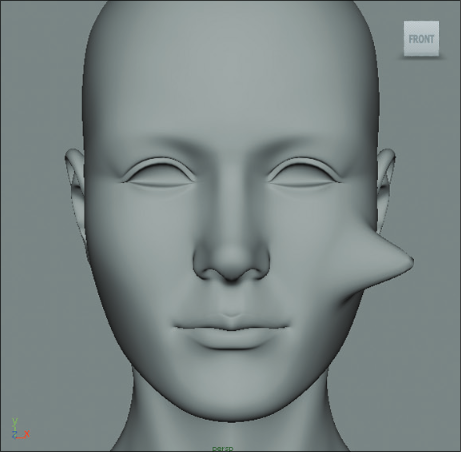
\includegraphics[scale=0.3]{img/unnatural_deformation.png}
  \end{subfigure}
  \caption{Unnatural Deformation.~\autocite{directmanipulationblendshapes}}
  \label{fig:unnaturaldeformation}
\end{figure}

To improve the model usability and prevent unnatural results,
the facial model can also be controlled through a set of parameters,
either chosen and implemented manually or automatically.

The (probably) first parametric face model was produced by F.I.\ Parke in 1974~\autocite{parametricface}:
It contains manually chosen parameters like \code{JAW ROTATION} (see \autoref{fig:parametricjawrotation}) or \code{MOUTH WIDTH} and applies different deformation operations like translation,
rotation or scaling on certain facial regions to realize them.

\begin{figure}[h]
  \centering
  \begin{subfigure}[b]{0.3\textwidth}
	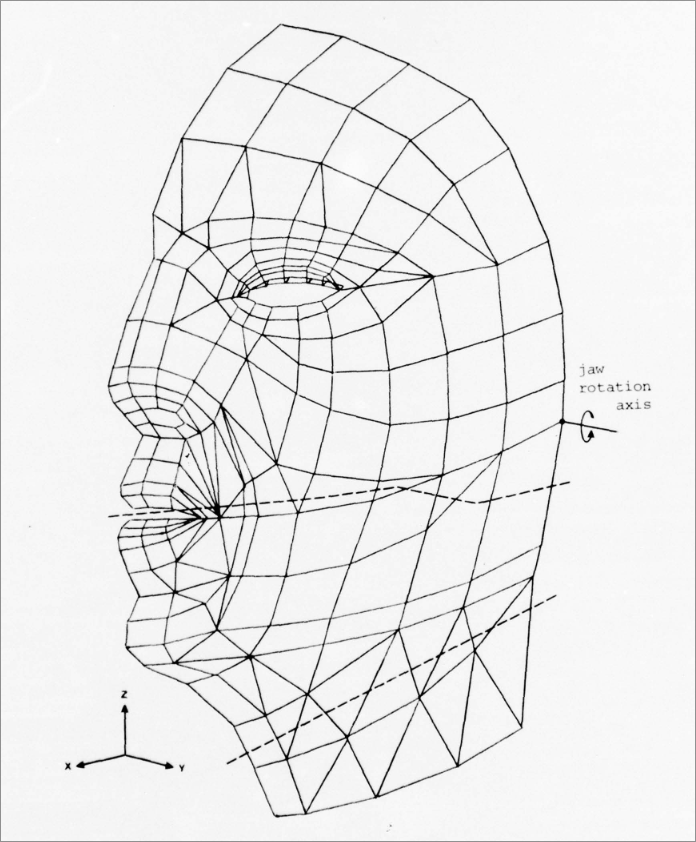
\includegraphics[scale=0.2]{img/parametric_model.png}
  \end{subfigure}
  \caption{Manually specified jaw rotation.~\autocite{parametricface}}
  \label{fig:parametricjawrotation}
\end{figure}

A different method to parameterize a face model is the \textquote{blend shape} approach:
Instead of using custom deformation operations on isolated parts of the mesh,
a blend shape model interpolates between different pre-modeled expressions that have identical vertex amounts and triangulation.
Multiple weighted expressions (\textquote{blend shape targets}) can be combined to generate the target expression.

By generating the target expression through a weighted sum of complete face models,
unwanted scale deformations can be introduced by choosing \textquote{wrong} weights.
Thus, the blend shape method was refined to combine local deviations from a neutral face instead,
called \textquote{delta blend shapes}.

Instead of manually associating each parameter with a certain expression,
model parameters can also be determined statistically,
e.g.\ by doing a principal component analysis of a range of facial expressions.
This generally results in non-interpretable model parameters,
which makes this model harder to animate,
as it is difficult to anticipate the resulting expression based on single parameter modifications.

It is also possible to apply more general character animation techniques like skeletal animation to faces,
as is often done in video games.
This approach is efficient to animate,
but weaknesses like unnatural skin and muscle movement become more significant in the case of faces,
so skeletal face animation might not be suitable if quality requirements are high.

Hybrid approaches,
like supplying a bone-driven model with a physical skin and muscle simulation,
can produce more realistic results,
but are also highly dependent on the character,
so the transfer of animations or \textquote{rigs} between characters might become difficult.
Also, physical simulation usually comes with a large performance impact,
which makes this technique unsuitable for real-time applications.

Skeletal rigs can also be combined with blend shapes,
as certain facial components that have a clear rotational axis (like eyes or jaw) are conveniently animated using a skeleton.
Blend shapes can then be used to correct skin movement or add detail.

\section{Kinematics}
\label{sec:kinematics}

Kinematics is a subfield of physics, dealing with the motion of bodies in a system while ignoring masses or forces.
A kinematic system in computer animation, like a skeleton, is modeled using rigid \textquote{bones} and rotatable \textquote{joints}\footnote{
  This differs for the blend shape approach,
  which is further described in \autoref{chap:blendshapemodels}.
}:

\begin{figure}[h]
  \centering
  \begin{subfigure}[b]{0.3\textwidth}
	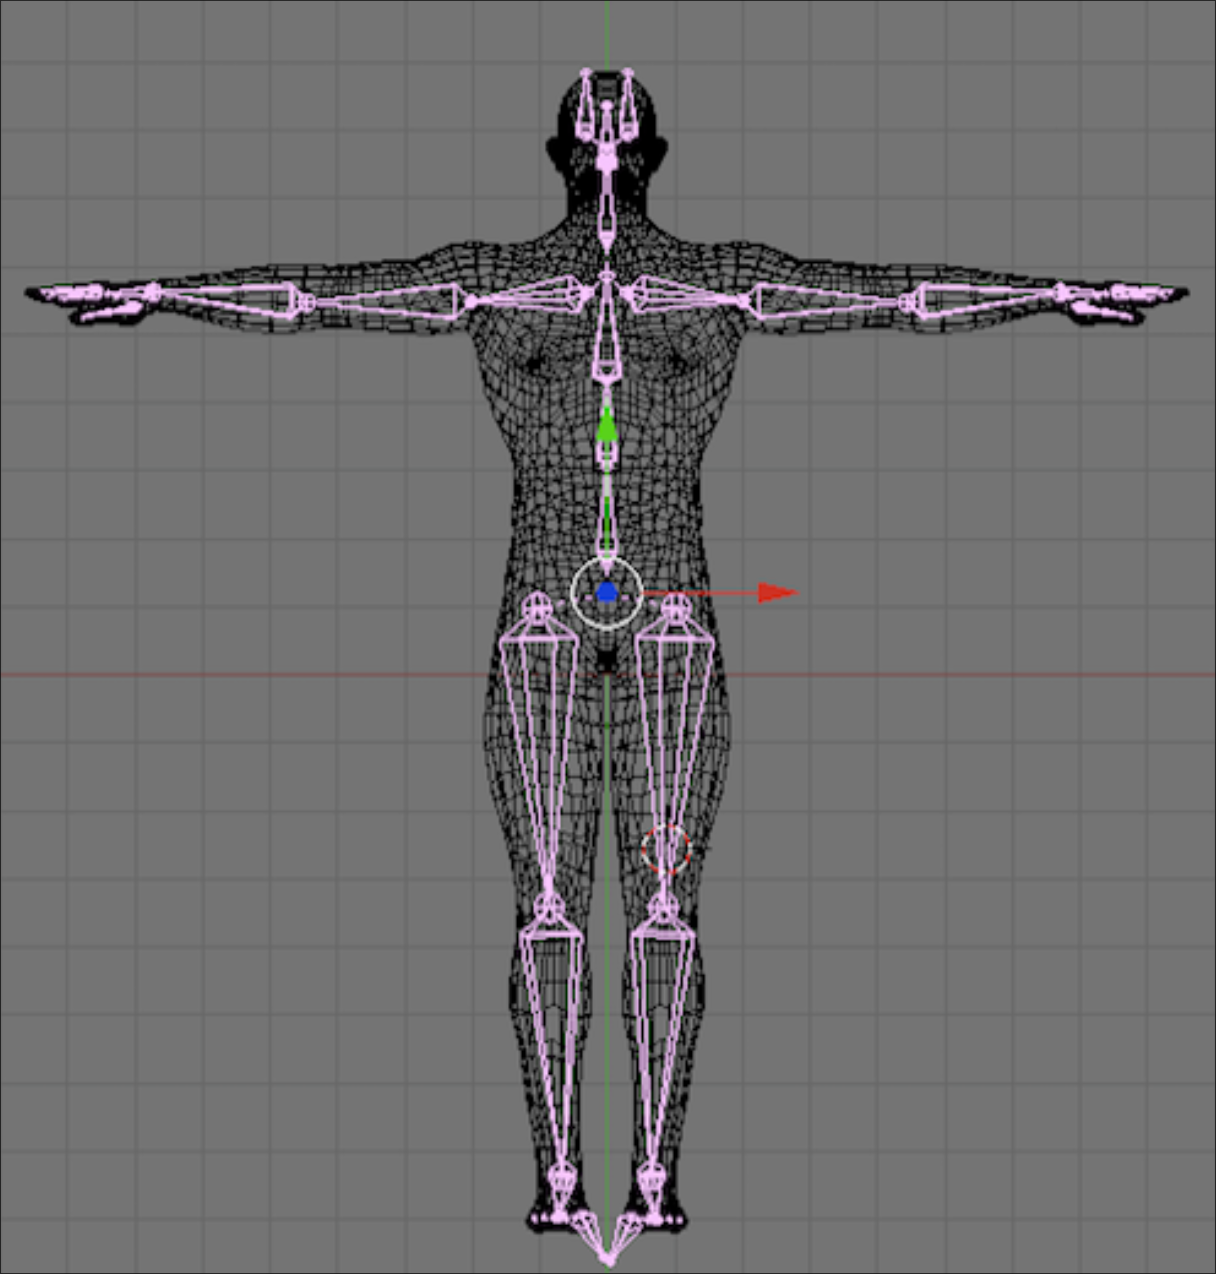
\includegraphics[scale=0.1]{img/human_rig.png}
  \end{subfigure}
  \caption{Human skeleton rig.~\autocite{computeranimation}}
  \label{fig:humanrig}
\end{figure}

The bones are ordered in a hierarchical relationship:
Rotating a single \textquote{parent} bone around its joint also rotates all \textquote{children} bones accordingly along the same center of rotation.
Controlling such a kinematic model can happen in two ways: Forward and inverse kinematics.

\textbf{Forward kinematics} calculates the absolute position of a joint (also called \textquote{end effector}) based on given joint orientations/angles of the parent joints.
In general, the forward kinematics problem can be expressed as \(x=f(\theta)\),
where \(x=(x_1,\dots,x_n)^T\) are the effector positions and \(\theta=(\theta_1,\dots,\theta_n)^T\) are the joint angles.

\textbf{Inverse kinematics} describes the opposite problem \(\theta=f^{-1}(x)\):
The absolute effector positions are given and the angles that produce these positions are to be determined.
Solving this problem for real-world models is difficult for multiple reasons:

\begin{itemize}
  \item High-quality kinematic models (e.g.\ for character animation) can have hundreds of degrees of freedom
  \item Multiple solutions or no solutions at all are possible
        (for a given \(x_2\) in \autoref{fig:2dforwardkinematics} there are two solutions for \(\theta\) already,
         as \(\theta_1\) and \(\theta_2\) can be exchanged)
  \item Different solutions can be ordered by criteria that are difficult to define analytically,
        for example by \textquote{intuitiveness} or if a solution is appropriate in the context of an animation
\end{itemize}

In consequence, approximative solvers are typically preferred over analytical ones.
 % Introduction
  \chapter{Skeletal Models}
\label{chap:skeletalmodels}

Pure skeletal kinematic models are typically used for body animation,
but they are also applicable to faces,
especially when quality requirements are not as important.
Quality issues when using skeletal models for facial animation are mostly rooted in the difficulty to obtain realistic skin movement when deforming a face by moving bones (e.g. through linear blend skinning or dual quaternion skinning).
Another problem is the model fidelity:
To be able to express sufficient details through animation,
a highly-detailed skeleton is required.
When a weakness is discovered during the animation process (for example when a certain expression can not be realized fully),
a skeletal model might be hard to adapt/improve without invalidating existing animations.
Despite these problems, skeletal animation may remain valid for faces,
for example when it is deployed in combination with other methods,
like blend shapes (discussed in \autoref{chap:blendshapemodels}).

\section{Skeletal Forward Kinematics}
\label{sec:skeletalforwardkinematics}

Skeletal forward kinematics is the problem
\[x=f(\theta),\]
where \(x\) are effector positions and \(\theta\) joint angles,
as described in \autoref{sec:kinematics}.

Take the following two-dimensional example (see \autoref{fig:2dforwardkinematics}) with two bones (green) and two \textquote{hinge}-joints (joints with a single degree of freedom, or a single rotational axis).

\begin{figure}[h]
  \centering
  \begin{subfigure}[b]{0.8\textwidth}
    \begin{tikzpicture}[scale=3]
      \clip (-1.5, -0.2) rectangle (2, 1.5);

      % Coordinates
      \coordinate (C) at (0, 0);
      \coordinate (X) at ({cos(30)}, {sin(30)});
      \coordinate (Y) at ({cos(30)}, 0);
      \coordinate (XX) at ({cos(30)+cos(60)}, {sin(30)+sin(60)});
      \coordinate (YY) at ($(X)+(30:{cos(30)})$); % Uses tikzlibrary "calc" for maths in ($...$)

      % Global axes
      \draw[>-stealth] (C) -- +(2, 0);
      \draw[>-stealth] (C) -- +(0, 1.5);

      % Circles
      % \draw[dashed] (0, 0) circle [radius=1];
      % \draw[dashed] (X) circle [radius=1];

      % Angle
      \draw (0.5, 0) arc[start angle=0, end angle=30, radius=0.5] node[left=0.1cm, below=0.15cm]{\footnotesize\(\theta_1\)};
      \draw ($(X)+(30:0.5)$) arc[start angle=30, end angle=60, radius=0.5] node[left, below=0.25cm]{\footnotesize\(\theta_2\)};

      % Bones
      \draw[green, very thick] (C) node[left, text=black]{\(x_1\)} -- node[above, text=black]{\(r_1\)} (X) node[below right, text=black]{\(x_2\)};
      \draw[green, very thick] (X) -- node[above, left, text=black]{\(r_2\)} (XX) node[above, text=black]{\(x_3\)};

      % Sine/Cosine sums
      \draw[blue, thick] ({cos(30)}, 0) -- node[below]{\footnotesize\(r_2\cos\theta_1+\theta_2\)} +({cos(60)}, 0);
      \draw[dashed] ({cos(30)+cos(60)}, 0) -- (XX);
      \draw[red, thick] (0, {sin(30)}) -- node[right]{\footnotesize\(r_2\sin\theta_1+\theta_2\)} +(0, {sin(60)});
      \draw[dashed] (0, {sin(30)}) -- (X);
      \draw[dashed] (0, {sin(30)+sin(60)}) -- (XX);

      % Sine/Cosine lines
      \draw[blue, thick] (C) -- node[below]{\footnotesize\(r_1\cos\theta_1\)} (Y);
      \draw[red, thick] (X) -- node[right]{\footnotesize\(r_1\sin\theta_1\)} (Y);
      \draw[blue, thick] (X) -- node[below, sloped]{\footnotesize\(r_2\cos\theta_2\)} (YY);
      \draw[red, thick] (XX) -- node[above, sloped]{\footnotesize\(r_2\sin\theta_2\)} (YY);

      % Local axes
      \draw[->, very thick] (C) -- +(30:0.3); % Polar coordinates
      \draw[->, very thick] (C) -- +(120:0.3);
      \draw[->, very thick] (X) -- +(60:0.3);
      \draw[->, very thick] (X) -- +(150:0.3);
    \end{tikzpicture}
  \end{subfigure}
  \caption{Simple 2D kinematic model.}
  \label{fig:2dforwardkinematics}
\end{figure}

To calculate the absolute position of \(x_3\) in the global coordinate system (the large one),
we can first look at the transformation at each joint individually and then trace the \textquote{bone-path} from the system's root to the end effector.
Describing \(x_3\) relative to the second joint's local coordinate system (the small one with its origin in \(x_2\)) is simple,
as its just a translation without rotation (\(x_{2\rightarrow 3}\) denotes the position of effector \(x_3\) relative to the coordinate system with origin in \(x_2\)):
\[x_{2\rightarrow 3}=\begin{pmatrix*}
  r_2\\
  0
\end{pmatrix*}.\]
To describe \(x_2\) relative to the first joint's local coordinate system (the small one with its origin in \(x_1\)),
we additionally have to consider to coordinate rotation caused by the second joint and the translation caused by the first bone (the one with length \(r_1\)).
The rotation is described using a two-dimensional rotation matrix \(R_2\) (\(2\times 2\) orthogonal matrix):
\[R_2=\begin{pmatrix*}
  &\cos\theta_2 &-\sin\theta_2\\
  &\sin\theta_2 &\cos\theta_2
\end{pmatrix*}.\]
The local translation caused by the first bone is
\[x_{1\rightarrow 2}=\begin{pmatrix*}
  r_1\\
  0
\end{pmatrix*},\]
it follows the affine transformation
\[x_{1\rightarrow 3}=x_{1\rightarrow 2}+R_2 x_{2\rightarrow 3}.\]
To obtain the global coordinates (denoted by just \(x_3\)), the rotation \(R_1\) caused by the first joint needs to be included (assuming the system has origin \((0, 0)\)):
\[x_3=R_1 x_{1\rightarrow 3}=R_1(x_{1\rightarrow 2}+R_2 x_{2\rightarrow 3}),\]
where
\[R_1=\begin{pmatrix*}
  &\cos\theta_1 &-\sin\theta_1\\
  &\sin\theta_1 &\cos\theta_1
\end{pmatrix*}.\]
Using addition theorems for sine and cosine, this leaves us with
\[x_3=\begin{pmatrix*}
  r_1\cos\theta_1+r_2(\cos\theta_1\cos\theta_2-\sin\theta_1\sin\theta_2)\\
  r_1\sin\theta_1+r_2(\sin\theta_1\cos\theta_2+\cos\theta_1\sin\theta_2)
\end{pmatrix*}=\begin{pmatrix*}
  r_1\cos\theta_1+r_2\cos(\theta_1+\theta_2)\\
  r_1\sin\theta_1+r_2\sin(\theta_1+\theta_2)
\end{pmatrix*},\]
which is also the intuitive solution when looking at \autoref{fig:2dforwardkinematics}.

\section{Skeletal Inverse Kinematics}
\label{sec:skeletalinversekinematics}

Skeletal inverse kinematics is the problem
\[\theta=f^{-1}(x).\]
As mentioned earlier, analytical solvers are rarely applied to this problem,
approximative solvers are usually used instead.
A starting approach is using the first order Taylor approximation of the effector's target positions \(t\):
\[t=f(\theta+\delta\theta)\approx f(\theta)+J(\theta)\delta\theta,\]
where \(J(\theta)\) is the Jacobian\footnote{
  \textquote{Jacobian entry \(J_{i, j}\) contains derivative of effector position \(x_i\) with respect to rotation angle \(\theta_j\) of joint \(j\)}.
}.
Solving for the angle-update \(\delta\theta\) yields the linear system
\[t-f(\theta)\approx J(\theta)\delta\theta,\]
which is (probably) difficult to solve because the system is usually underconstrained, \(J(\theta)\) might not be invertible or maybe there is no solution at all (for example if the target positions are out of reach of the effectors).

The approximative target to minimize to obtain a \(\delta\theta\) that best satisfies \(t-f(\theta)\approx J(\theta)\delta\theta\) when the inverse kinematics problem doesn't have a solution is the \textbf{least squares} solution
\[\delta\theta=\arg\min\limits_{\delta\theta}||J(\theta)\delta\theta-(t-f(\theta))||^2.\]
The target to minimize to obtain a \(\delta\theta\) that satisfies \(t-f(\theta)=J(\theta)\delta\theta\) when the inverse kinematics problem has a single or multiple solutions is the \textbf{least norm} solution
\[\delta\theta=\arg\min\limits_{\delta\theta}||\delta\theta||,\]
such that \(t-f(\theta)=J(\theta)\delta\theta\).

\subsection{Moore-Penrose Inverse}
\label{subsec:moorepenroseinverse}

A generally possible \textquote{best-effort} solution to linear systems with no/infinitely many solutions is given by the \textbf{Moore-Penrose Inverse}:
When solving a linear system \(Ax=b\) using \(x=A^{-1}b\) is not possible (e.g. because \(A\) is not invertible),
calculate \(x\approx A^+b\) instead, where \(A^+\) is the Moore-Penrose inverse (or \textquote{pseudo-inverse}).
If the system is overconstrained, this approach minimizes \(||Ax-b||^2\) (least squares),
if the system is underconstrained, it minimizes \(||x||\) (least norm) such that \(Ax=b\),
and if \(A\) is actually invertible, \(A^+=A^{-1}\).

The pseudo-inverse can be calculated using a singular-value-decomposition:
Inverting a regular invertible matrix \(A=U\Sigma V^T\), \(A\in\mathbb{R}^{n\times n}\) yields
\[A^{-1}=(U\Sigma V^T)^{-1}=(V^T)^{-1}\Sigma^{-1}U^{-1}=V\Sigma^{-1}U^T\]
with \(\Sigma^{-1}=\text{diag}(\frac{1}{\lambda_1},\dots,\frac{1}{\lambda_n})\),
\textquote{pseudo-inverting} a non-invertible matrix \(A=U\Sigma V^T\), \(A\in\mathbb{R}^{n\times n}\) with \(\text{rank}(A)=m<n\) yields
\[A^+=(U\Sigma V^T)^+=(V^T)^+\Sigma^+U^+=(V^T)^{-1}\Sigma^+U^{-1}=V\Sigma^+U^T\]
with \(\Sigma^+=\text{diag}(\frac{1}{\lambda_1},\dots,\frac{1}{\lambda_m},0,\dots,0)\).

Using the pseudo-inverse, the inverse kinematics problem can now be solved by iteratively updating the joint angles \(\theta\) in direction of \(\delta\theta=J(\theta)^+(t-f(\theta))\).
 % Skeletal models
  \chapter{Blend Shape Models}
\label{chap:blendshapemodels}

Facial animation in film is typically done using blend shape models,
as they provide an easy-to-use framework that disallows unnatural facial deformations (unlike e.g.\ freeform deformations),
while also exposing parameters that are intuitively interpretable by animators (unlike e.g.\ generative PCA models).
A blend shape model is a linear, \textbf{semantic parameterization} of a face's range of expressions,
where the individual components (the \textbf{blend shape targets}) are \textquote{core} expressions that are linearly combined to reach a greater range of \textquote{mixed} expressions (the blend shape targets are the \textquote{basis} of the spanned \textquote{expression-space}).
This choice of linear components introduces a semantic interpretability to the model parameters,
as each parameter controls the influence of an intuitive human expression on the resulting model.
The total \textquote{range} of the model depends on the number of used blend shapes,
but in general a blend shape model remains a lossy representation of the human expression-space.

Custom blend shape targets can be chosen depending on the model requirements,
with the \textquote{Facial Action Coding System} (FACS) there also exists a standardized definition of \textquote{components} of facial expressions based on human anatomy.
FACS defines 46 \textquote{action units} that correspond to facial muscle movements (not counting units for general head and eye movement),
which can be realized as delta blend shape targets.

In contrast to skeletal forward and inverse kinematics,
blend shape kinematics does not deal with models made of bone segments and joints,
although the general problem formulations \(x=f(\theta)\) (forward) and \(\theta=f^{-1}(x)\) (inverse) stay the same.

\section{Delta Blend Shape Forward Kinematics}
\label{sec:blendshapeforwardkinematics}

The forward kinematics approach to facial animation using delta blend shape models consists of an animator tuning individual parameters of the model to reach a target expression.
The blend shape model's components are the \textquote{neutral face} \(b_0\) and \(n\) blend shape targets (custom created facial expressions) \(b_1,\dots,b_n\) (\(b_i\) always denotes a regular blend shape target, delta blend shape targets are denoted as \(b_i-b_0\)).
Each \(b_i\) has \(m\) vertices and identical triangulation to allow representation of a target expression as a linear combination of \(b_0,\dots,b_n\).
Every blend shape \(b_i\) \textquote{is a vector of \(m\) stacked vertex positions}:
\[b_i=\begin{pmatrix}
  x_i^{(i)}\\
  \vdots\\
  x_m^{(i)}\\
\end{pmatrix}\in\mathbb{R}^{3m}.\]
Because \(x_i^{(i)}\in\mathbb{R}^3\),
each vertex's three coordinates are contained in \(b_i\) either in packed or interleaved fashion:
\(b_i=(x_1,\dots, x_m, y_1,\dots,y_m, z_1,\dots, z_m)^T\) or \(b_i=(x_1,y_1,z_1,\dots,x_m,y_m,z_m)^T\).
The ordering does not matter, as long as it is identical for every \(b_i\) and the neutral face \(b_0\).

A target expression \(F(w)\) is then generated by setting the \(n\)-dimensional parameter-vector \(w\) for an affine linear combination:
\[F(w)=b_0+\sum\limits_{i=1}^n w_i(b_i-b_0).\]
By combining divergences from the neutral face (\textquote{delta-blend shapes}),
each parameter \(w_i\) can be chosen arbitrarily\footnote{
  Parameters should be chosen from the interval \([0, 1]\).
  For the inverse kinematics problem,
  this range is usually not enforced,
  since the target expression could leave the spanned expression space (for example by opening the mouth too much).
  For slight excesses this shouldn't be a problem,
  but in general the delta blend shape target \(b_i\) is reached fully with weights \(w_j=0\ \forall j\neq i\) and \(w_i=1\),
  so a weight exceeding \(1\) is of undefined quality.
},
while the effective weights \(\alpha_0,\dots,\alpha_n\) for blend shapes \(b_0,\dots,b_n\) still satisfy the affine property \(\sum_{i=0}^n\alpha_i=1\) (which is required,
otherwise the target expression could \textquote{leave} the expression space spanned by the blend shapes,
for example by unwanted scale deformations):
\begin{align*}
  F(w)&=b_0+\sum\limits_{i=1}^{n}w_i(b_i-b_0)\\
  &=b_0+\sum\limits_{i=1}^{n}w_i b_i-\sum\limits_{i=1}^{n}w_i b_0\\
  &=b_0\underbrace{\left(1-\sum\limits_{i=1}^{n}w_i\right)}_{\alpha_0}+\sum\limits_{i=1}^{n}\underbrace{w_i}_{\alpha_i} b_i\\
  \Rightarrow \sum\limits_{i=0}^{n}\alpha_i &= 1-\left(\sum\limits_{i=1}^{n}w_i+\sum\limits_{i=1}^{n}w_i\right)=1
\end{align*}
By combining the delta blend shape vectors \(b_i-b_0\) into a matrix
\[B=[b_1-b_0|\dots|b_n-b_0]\]
with \(B\in\mathbb{R}^{3m\times n}\), the model can be formulated more compactly:
\[F(w)=b_0+Bw.\]

The semantic nature of blend shape models makes animation using this forward approach generally possible for smaller models,
but it becomes inefficient or even impossible for high-quality models with hundreds of parameters\footnote{
  The facial model created for \textquote{Gollum} from \textquote{The Lord of the Rings} uses over \(900\) blend shape targets.~\autocite{computeranimation}
}.

\section{Delta Blend Shape Inverse Kinematics}
\label{sec:blendshapeinversekinematics}

For this reason, animation using the inverse kinematics approach is desirable:
Instead of interacting with individual parameters,
\textquote{markers} or \textquote{manipulators} are placed on the model,
which allow to define the target expression more directly.
Markers positions can be obtained either manually through a user interface which allows direct interaction with the model (like in \autoref{fig:effectorface}) or through facial tracking (see \autoref{chap:performancedrivenfacialanimation}).
The blend shape parameters are then determined to match this target expression as closely as possible.

\begin{figure}[h]
  \centering
  \begin{subfigure}[b]{0.53\textwidth}
	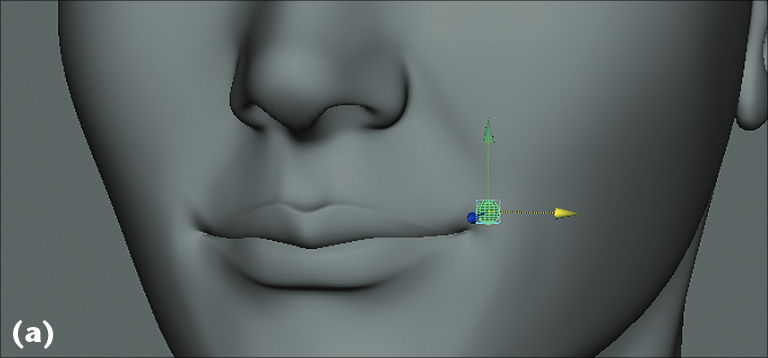
\includegraphics[scale=0.3]{img/effector_face.png}
  \end{subfigure}
  \caption{A marker placed on a facial model.~\autocite{directmanipulationblendshapes}}
  \label{fig:effectorface}
\end{figure}

Placing a marker on the model effectively means choosing a vertex,
whose position should act as a constraint for the face deformation.
Marker \(i\)'s current position is the current vertex position \(x_i\),
which depends on the current model parameters \(w\).
The vertex's target position \(t_i\) can then be defined by moving the marker around.

Determining the model parameters \(w\) to satisfy the marker constraints can be formulated as the following minimization problem:
\[w=\arg\min\limits_w||\overline{B}w-(\overline{t}-\overline{b}_0)||^2=\arg\min\limits_w||\overline{B}w-m||^2,\]
where \(t\) is the vector of all marker's target positions,
\(m\) are the offsets of the target positions from the neutral face (offsets are used because of delta blend shapes) and \(\overline{B}\),
\(\overline{t}\) and \(\overline{b}_0\) correspond to \(B\),
\(t\) and \(b_0\) but only contain the rows belonging to the vertices that are constrained by markers.~\autocite{directmanipulationblendshapes}
This means, \(\overline{B}\) contains \(3\) rows for each placed marker.
Since the direct manipulation allows targeting expressions outside the model's expression space,
an exact solution is generally not possible.
Also, the above minimization problem will be under-constrained in most cases (unless the animator places possibly hundreds of markers),
so additional constraints or regularization terms need to be introduced.

To improve temporal continuity of the animation, weight differences between updates can be minimized by introducing \(\alpha||w-w_0||^2\) to the problem,
where \(w_0\) are the previous weights:~\autocite{directmanipulationblendshapes}
\[w=\arg\min\limits_w||\overline{B}w-m||^2+\alpha||w-w_0||^2,\]
Lewis and Anjyo add \(\mu||w||^2\) as another regularization term,
with the intention to oppose \textquote{extreme} solutions,
for example caused by weight growth due to numerical errors in \textquote{oscillating} animations:~\autocite{directmanipulationblendshapes}
\[w=\arg\min\limits_w||\overline{B}w-m||^2+\alpha||w-w_0||^2+\mu||w||^2.\]
This term is also important since the weights \(w\) are not constrained to \([0, 1]\) for the inverse problem (at least not in this solution).

The parameters \(\alpha\) and \(\mu\) are set to small values to not significantly alter the main objective,
Lewis and Anjyo use \(\alpha=0.1\) and \(\mu=0.001\).~\autocite{directmanipulationblendshapes}

\section{Solving the Inverse Kinematics Minimization Problem}
\label{sec:solvingblendshapeinversekinematics}

The goal is the minimization of
\[||\overline{B}w-m||^2+\alpha||w-w_0||^2+\mu||w||^2,\]
which is quadratic in \(w\).
Since we are using the euclidian norm,
it follows that
\[||x||^2=\sqrt{x_1^2+\dots+x_n^2}^2=x_1^2+\dots+x_n^2=x^T x\]
for \(x\in\mathbb{R}^n\), which allows us to rewrite the term as
\begin{align*}
  &(\overline{B}w-m)^T(\overline{B}w-m)+\alpha(w-w_0)^T(w-w_0)+\mu w^T w\\
  =\ &(w^T \overline{B}\,^T \overline{B}w-2w^T \overline{B}\,^T m+m^T m)\\
  &+\alpha(w^T w-2w^T w_0+w_0^T w_0)\\
  &+\mu(w^T w).
\end{align*}
Deriving this (using some slightly sketchy matrix differential notation\footnote{
  Sketchy example:\\
  \(d\phi(w)=d(w^T\overline{B}\,^T\overline{B}w)=(dw)^T\overline{B}\,^T\overline{B}w+w^T\overline{B}\,^T\overline{B}(dw)=2w^T\overline{B}\,^T\overline{B}(dw)\Leftrightarrow\frac{d\phi}{dw}=2\overline{B}\,^T\overline{B}w\)
}) leads to the following derivative:
\[2\overline{B}\,^T\overline{B}w-2\overline{B}\,^T m+2\alpha w-2\alpha w_0+2\mu w.\]
Solving for \(0\) to find the local extremum leads to
\begin{align*}
  2\overline{B}\,^T\overline{B}w+2\alpha w+2\mu w&=2\overline{B}\,^T m+2\alpha w_0\\
  \Leftrightarrow\left(\overline{B}\,^T\overline{B}+(\alpha+\mu)I\right)w&=\overline{B}\,^T m+\alpha w_0,
\end{align*}
which is a \(n\times n\) linear system (\(n\) is the number of blend shapes/model parameters),
where \(I\in\mathbb{R}^{n\times n}\) is the identity matrix.
The above condition is sufficient, since the problem is convex.

Because \(\overline{B}\,^T\overline{B}\) and \((\alpha+\mu)I\) are both (usually) positive definite\footnote{
  For a matrix \(A\), \(A^T A\) is positive definite if \(Ax\neq 0\) for any non-zero vector \(x\),
  since \(x^T A^T Ax=(Ax)^T(Ax)=||Ax||^2\).
  This is probably true for \(\overline{B}\),
  since \(\overline{B}\)'s columns (the partial delta blend shape targets) should be linearly independent.
}\ \footnote{
  The identity matrix and its scalar multiples are positive definite.
} and equal to their (conjugate\footnote{
  We only deal with real numbers (coordinates from \(\mathbb{R}^3\)).
}) transposes\footnote{
  \((A^T A)^T=A^T(A^T)^T=A^T A\).
}, an efficient Cholesky solver can be applied to obtain \(w\).~\autocite{computeranimation}

\subsection{Inverse Kinematics Instability}
\label{subsec:pseudoinverseinstability}

Disregarding implementation-specific numerical instabilities and assuming that \(\overline{B}\) is invertible because all delta blend shape targets are linearly independent\footnote{
  If \(\exists\ i, w: b_i = \sum\limits_{j\neq i} w_j b_j\), \(b_i\) can be removed, as it does not add information to the model.
} (so \(\overline{B}\) has full rank),
we have the following equivalence:

\[
  \left(\overline{B}\,^T\overline{B}+(\alpha+\mu)I\right)w=\overline{B}\,^T m+\alpha w_0
  \Leftrightarrow w=\left(\overline{B}\,^T\overline{B}+(\alpha+\mu)I\right)^{-1}\left(\overline{B}\,^T m+\alpha w_0\right)
\]

This is a (regularized) Moore-Penrose pseudo-inverse\footnote{
  This is only true if \(\overline{B}\)'s columns are linearly independent, which I will assume from now on.
  Under these circumstances, it follows for a full-rank matrix \(A\):
  \begin{align*}
    A&=U\Sigma V^T=U\left((\Sigma^+)^T\Sigma\right)\Sigma V^T=U(\Sigma^+)^T (V^T V)\Sigma (U^T U)\Sigma V^T\\
    &=(V\Sigma^+ U^T)^T(U\Sigma V^T)^T(U\Sigma V^T)=\left((U\Sigma V^T)^+\right)^T(U\Sigma V^T)^T(U\Sigma V^T)\\
    &=(A^+)^T A^T A\Leftrightarrow A^T=(A^T A) A^+\Leftrightarrow A^+=(A^T A)^{-1}A^T.
  \end{align*}
  Full rank is required for the property \((\Sigma^+)^T\Sigma=I\).
} or \textquote{damped-least-squares} method:
If we set \(\alpha=0\) and \(\mu=0\) we obtain

\[w=\left(\overline{B}\,^T\overline{B}\right)^{-1}\overline{B}\,^T m=\overline{B}\,^+ m.\]

This can lead to instabilities when \textquote{dragging} or animating a placed marker/constraint:~\autocite{transpositiondirectmanipulationblendshapes}
If we expand our forward kinematics problem \(F(w)=b_0+Bw\) using a singular value decomposition, we end up with

\[F(w)=b_0+U\Sigma V^T w,\]

where the largest singular values in \(\Sigma\) will have the most influence on the generated facial expression.
These are the values that should mainly be used to solve the inverse kinematics problem.

Now, looking at the singular value decomposition of the unregularized inverse kinematics problem \(w=\overline{B}\,^+ m\), we obtain

\[w=(U\Sigma V^T)^+ m=(V^T)^+\Sigma^+U^+ m=V\Sigma^+U^T m,\]

because \(V\) and \(U\) are orthogonal matrices\footnote{
  \(U^+=U^{-1}=U^T\).
}.

Since we take the pseudo-inverse \(\Sigma^+\),
the non-zero diagonal entries of \(\Sigma\) are inverted,
which means this inverse kinematics solution is influenced strongly by the smaller singular values from the forward kinematics problem.
In consequence, the facial deformations produced to satisfy a marker constraint might also occur outside this marker's local environment\footnote{
  In some cases this might be even desirable,
  for example when a smile produces deformations in the eye-region,
  but this makes the model slightly unpredictable.
}, which could lead to inconsistencies during animation.

A possible solution is given by the transposition-based solution of the inverse kinematics problem.~\autocite{transpositiondirectmanipulationblendshapes}~\autocite{jacobiantranspose}

\section{Corrective and Intermediate Blend Shapes}
\label{sec:correctiveblendshapes}

Although the \textquote{basis vectors} of the spanned expression space (the blend shape targets) are valid facial expressions,
arbitrary linear combinations can still produce unnatural anomalies.

\begin{figure}[h]
  \centering
  \begin{subfigure}[b]{0.25\textwidth}
	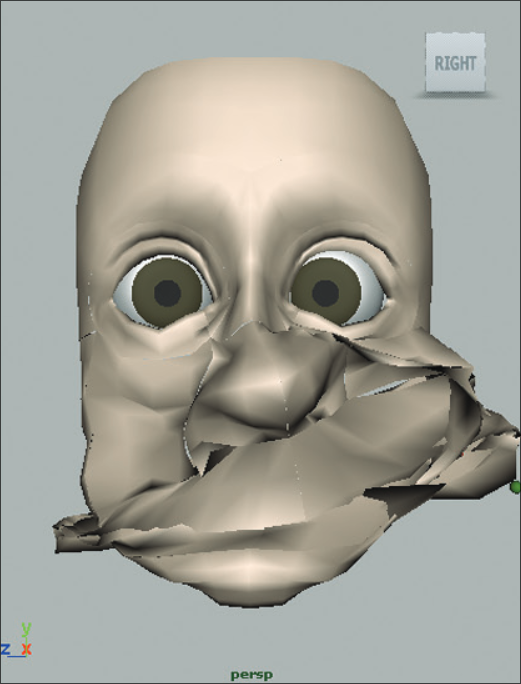
\includegraphics[scale=0.2]{img/unconstrained_weights.png}
  \end{subfigure}
  \caption{Consequences of unconstrained blend shape weights.~\autocite{directmanipulationblendshapes}}
  \label{fig:unconstrainedweights}
\end{figure}

For this reason, \textquote{corrective} blend shapes are used:
By adding blend shape targets with additional weights (not part of the manual model parameters) that depend on other weights,
anomalies caused by special weight combinations can be fixed.

For example, if an anomaly occurs when activating weights \(w_j\) and \(w_k\) for blend shape targets \(b_j\) and \(b_k\),
a corrective blend shape \(b_{(j,k)}\) (\textit{not} in delta blend shape form!) can be modeled for the expression produced by the weights \(w_j=w_k=1\) and \(w_i=0\ \forall i\notin\{j, k\}\).
By setting the weight to \(w_{(j,k)}=w_j\cdot w_k\), the blend shape automatically activates when both \(b_j\) and \(b_k\) become active.

The resulting blend shape model is quadratic with respect to its parameters \(w\):
\begin{align*}
  F_C(w)&=F(w)+\sum\limits_{(i,j)\in C}w_{(i,j)} b_{(i,j)}\\
      &=b_0+\sum\limits_{i=1}^{n}w_i(b_i-b_0)+\sum\limits_{(i,j)\in C}w_i w_j b_{(i,j)},
\end{align*}
where \(C=\{1,\dots,n\}\times\{1,\dots,n\}\) and \(b_{(i,j)}\) denotes the corrective blend shape for blend shape targets \(b_i\) and \(b_j\).
Because of the quadratic nature of this model,
the inverse kinematics problem can no longer be solved by a simple convex optimization.
A possible solution for the quadratic case is given in~\autocite{nonconvexblendshapes},
although corrective blend shapes could also be applied in a third-order fashion or higher (correcting anomalies caused by three or more overlapping blend shape targets).

Another problem arises from the linear nature of the blend shape model:
Certain rotational movements like closing eyelids or eye rotations can only be represented in a linear fashion.
When animating an eyeball movement (like a gaze from center to right),
the eyeball will loose a part of its volume in the first half of the animation and regain it in the second half,
since each individual vertex can only move in a straight line.
To solve this problem, \textquote{intermediate} blend shapes are used:
An additional blend shape target is modeled for a single (or multiple) intermediate animation state(s),
leading to a piecewise linear interpolation/approximation (see \autoref{fig:combinationvsintermediate}).

\begin{figure}[h]
  \centering
  \begin{subfigure}[b]{0.45\textwidth}
	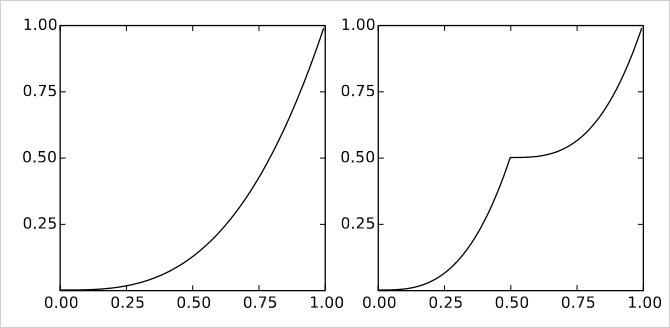
\includegraphics[scale=0.3]{img/combination_vs_intermediate.png}
  \end{subfigure}
  \caption{Corrective blend shapes lead to smooth interpolation that becomes significant if all weights approach \(1\) (left),
    intermediate blend shapes lead to non-smooth interpolation (right).~\autocite{practicetheoryblendshapes}
  }
  \label{fig:combinationvsintermediate}
\end{figure}

This approach can be handled by the in \autoref{sec:blendshapeinversekinematics} described inverse kinematics solution,
as intermediate blend shapes are just appended to the existing linear model.

\section{Combining Skeletal and Blend Shape Animation}
\label{sec:combiningskeletalandblendshapes}

Instead of using intermediate blend shapes to better approximate rotational deformations,
certain facial movements like eye-, eyelid- or jaw rotations can be modeled using skeletal animation and skinning\footnote{
  \textquote{Skinning} is the translation of abstract bone movements into actual skin/vertex movements.
}.
This does not require modeling all facial animation using bones,
as blend shape animation and skeletal animation can be combined.

To achieve this, the blend shape inverse kinematics problem is solved first,
as the deformations caused by skinning do not match the blend shape targets.
The skeletal inverse kinematics problem can be solved later,
because vertex deformations caused by the blend shape model do not modify bone positions.

Although this approach might achieve better performance with rotational movement,
the resulting expressions loose some control,
as the interactions between blend shape and skinning deformations are unclear\footnote{
  It is unclear to me if this model is viable.
}.

A different combinational model is possible by applying corrective blend shapes to a primarily skeleton-based model:
In cases where memory availability is low,
skeletal models may be preferred over blend shape models\footnote{
  Skeletal models are more taxing on CPU/GPU computations,
  since skinning is more computationally expensive than linear interpolation.
  Blend shape models are more taxing on CPU/GPU memory (especially for detailed models with many blend shapes or situtations with many different characters with their own blend shapes),
  since the face is stored many times with different deformations (although data blend shapes help here, as the localized deformations lead to sparse delta blend shape targets).
}.
To still achieve realistic skin movement (which might be hard only through skinning),
corrective blend shapes can be applied after the skinning,
with weights depending on certain joint angles.
In that case, only skeletal inverse kinematics is involved.
 % Blend shape models
  \chapter{Performance Driven Facial Animation}
\label{chap:performancedrivenfacialanimation}

Facial animation is rarely a fully manual process,
either for efficiency reasons as manual animation is a work-intensive process,
or to capture more true-to-life facial expressions,
or in case of real-time applications,
where manual animation is not applicable at all.
Classical face tracking used in film or video games is typically marker-based optical tracking,
but with the emergence of head-mounted technology like virtual- or augmented-reality headsets,
this method is no longer fitting,
because a large part of the face is obstructed when wearing head-mounted displays.

\section{Stereo/Optical Facial Tracking}
\label{sec:facialtracking}

Marker-based face tracking (or motion capture in general) works similar to stereo 3D-scanning:
At least two cameras point at the face to be tracked,
which is augmented with \textquote{markers} (easily identifiable points),
so facial features can be reliably tracked by all cameras.
Because cameras can \textquote{see} the same marker from multiple perspectives (the camera positions have to be known),
the distance of a marker from both cameras can be calculated by solving the intersection of the straight lines defined by each camera position and the marker position.
In the schematic in \autoref{fig:2dstereotracking}, the cameras are marked blue, while the marker on the face is marked red.

\begin{figure}[h]
  \centering
  \begin{subfigure}[b]{0.75\textwidth}
    \begin{tikzpicture}[scale=3]
      \clip (-2, -0.2) rectangle (3, 1.3);

      % Coordinates
      \coordinate (CA) at (-1, 0);
      \coordinate (CB) at (1, 0);
      \coordinate (M) at (0, 1);

	  % Axis
	  \draw[->] (-1.5, 0) -- (1.5, 0); % x
	  \draw[->] (0, 0) -- (0, 1.3); % y

      % Cameras
      \node[isosceles triangle, isosceles triangle apex angle=30, draw, fill=blue, minimum size=0.5, rotate=225] (TA) at (CA){};
      \node[isosceles triangle, isosceles triangle apex angle=30, draw, fill=blue, minimum size=0.5, rotate=315] (TB) at (CB){};

	  % Camera beams
	  \draw[->, blue] (CA) -- (M) -- +(0.2, 0.2);
	  \draw[->, blue] (CB) -- (M) -- +(-0.2, 0.2);

	  % Marker
	  \draw[fill=red] (M) circle (0.025);

      % Face
      \draw[green] (M) +(0, 0.05) circle (0.2);
      \draw[green] (M) +(0.075, 0.1) circle (0.04);
      \draw[green] (M) +(-0.075, 0.1) circle (0.04);
      \draw[green] (M) +(-0.075, -0.075) arc[start angle=225, end angle=315, radius=0.1]{};
    \end{tikzpicture}
  \end{subfigure}
  \caption{2D Stereo Tracking.}
  \label{fig:2dstereotracking}
\end{figure}

When basic information about the camera is known (e.g. focal length and sensor size),
the beam directions can be inferred from the marker's pixel position in the image plane.
This allows defining straight line equations for both beams,
equating those and solving the resulting linear system leads to the distance from the camera.
Because the camera positions are known, the marker's position is also known.

By adding more cameras to the tracking setup and thus increasing the size of the linear system to be solved,
errors can be reduced and the tracking area increased (surround cameras also enable tracking rotations).
Proprietary tracking systems like OptiTrack~\autocite{optitrack} use techniques like infrared cameras with infrared emitters and reflective markers
to lessen the influence of regular daylight and simplify the marker detection.

Finally, when the marker positions have been calculated,
the inverse kinematics problem for either blend shapes or a skeleton can be solved,
since each marker corresponds to a vertex of the facial model.

\section{Tracking Solutions in Consumer VR Products}
\label{sec:consumertrackingsolutions}

Because head-mounted-displays hinder the application of facial markers,
facial tracking data for a portion of a face is typically extracted from a single camera feed instead of multiple.
Cameras might be mounted inside the HMD, facing the eyes and nose, and below the HMD, facing the mouth and chin.
Since a delta blend shape model linearly combines locally isolated deformations,
processing different facial regions individually does not impose a problem.

Unlike the stereo tracking, this approach does not use the inverse kinematics method described in \autoref{sec:blendshapeinversekinematics}.
Instead, each camera feed is fed through a specialized computer vision model,
which directly calculates the blend shape weights for a particular facial region and blend shape model.
 % Performance capture

  % \begin{appendices}
  %   \chapter{Appendix 1}
\label{ch:appendix1}

% Chapter Introduction

\clearpage

\section{Section 1}
\label{sec:appendixsection1}

% Section Text

\cleardoublepage
  % \end{appendices}

\end{thesis}
\end{document}